\RequirePackage[l2tabu,orthodox]{nag} % This package helps prevent you from doing things wrong.

\documentclass[10pt,a4paper]{article}

\usepackage{ifluatex}
\ifluatex
\usepackage{fontspec}
\usepackage{unicode-math}

%\setmainfont[Ligatures=TeX]{xits}
%\setmathfont[math-style=ISO]{xits-math}
\setmainfont[Ligatures=TeX]{Latin Modern Roman}
\setmathfont[math-style=ISO]{lmmath-regular.otf}
\else
\usepackage[utf8]{inputenc}
\fi

\usepackage[margin=2cm,includefoot]{geometry}
\usepackage{amsmath, mathtools, cancel}
\usepackage{graphicx, subfig, float, grffile}
\usepackage{algorithm,algorithmic}
\usepackage{microtype}
\usepackage{todonotes}
%\usepackage[firstinits=true, style=alphabetic, url=false, isbn=false, hyperref=true]{biblatex}
%\def\bibfont{\footnotesize}
\usepackage{siunitx}
\usepackage{tikz}
\usepackage{pgfplots}

%\usepackage{hyperref}
\usepackage{cleveref}
%\usepackage[T1]{fontenc}

%\usepackage[width=0.7\paperwidth,height=0.85\paperheight]{geometry}
\linespread{1.3}
\usepackage{contmech}
\ifluatex
  \renewcommand{\ta}[1]{\mathbfit{#1}}
  \renewcommand{\ts}[1]{\mathbfit{#1}}
  \renewcommand{\td}[1]{\mathbfcal{#1}}
  \renewcommand{\tf}[1]{\mathbfsfup{#1}}
  \renewcommand{\Box}{\mdlgwhtsquare}
  \renewcommand{\leadsto}{\rightsquigarrow}
\fi
% \renewcommand{\vec}[1]{\mathds{#1}}
% \renewcommand{\mat}[1]{\mathds{#1}}

\captionsetup[subfigure]{textfont=it}
\captionsetup[figure]{textfont=it}
\newcommand{\figref}[1]{Figure~\ref{#1}}

\renewcommand{\topfraction}{1.0}	% 99% of page top can be a float
\renewcommand{\bottomfraction}{1.0}	% 99% of page bottom can be a float
\renewcommand{\textfraction}{0.0}	% only 1% of page must to be the text
\renewcommand{\floatpagefraction}{1.0} % 99% of whole page can be a float
\setcounter{totalnumber}{100} %maximum floating objects on one page

% More specialized commands;
\DeclarePairedDelimiter{\homogenized}{\langle}{\rangle}
\newcommand{\fluid}{\mathrm{part}}
\newcommand{\pore}{\mathrm{pore}}
\newcommand{\particle}{\mathrm{part}}
\newcommand{\free}{\mathrm{f}}
\newcommand{\prescribed}{\mathrm{p}}
\newcommand{\moving}{\mathrm{mov}}
\newcommand{\segment}{\mathrm{segm}}
\newcommand{\corner}{\mathrm{corn}}
\newcommand{\contact}{\mathrm{cont}}
\newcommand{\external}{\mathrm{ext}}
\newcommand{\internal}{\mathrm{int}}
\newcommand{\surf}{\mathrm{s}}
\newcommand{\mesh}{\mathcal{M}}
\newcommand{\on}{\quad\text{ on }}
\newcommand{\NDIM}{n_\mathrm{dim}}
\newcommand{\tang}{\mathrm{T}}
\newcommand{\curve}{\mathcal{C}}

\newcommand{\ded}{\mathrm{d}}
\newcommand{\dep}{\mathrm{p}}

%\newcommand{\on}{\mid}
%\newcommand{\surfdiff}{\hat{\ts\nabla}}
%\newcommand{\at}[2]{\left.#1\right|_{#2}}

\begin{document}
\title{FE$^2$ for Liquid-Phase Sintering with Seamless Transition from Macroscopic Compressibility to Incompressibility}

\author{
Mikael Öhman, Fredrik Larsson and Kenneth Runesson\\
Department of Applied Mechanics \\
Chalmers University of Technology}

\maketitle

\begin{abstract}
\noindent In a previous paper, \textsc{Öhman et al.} \cite{OhmanRunLar2011}, liquid phase sintering of particle agglomerates was modeled on the mesoscale as the viscous deformation of particle-particle contact, whereby the single driving force is the surface tension on the particle/pore interface. A FE\textsuperscript{2}-strategy was outlined; however, the variational setting is applicable only under the restriction of non-vanishing macroscopic porosity (corresponding to a not fully dense end-product). The present paper generalizes this situation such that it allows for the transition to zero porosity, which is accomplished by introducing a mixed variational format of the macroscale problem. This has consequences also for the formulation of the RVE-problem, that is complemented with an extra constraint equation regarding the prolongation of the volumetric part of the macroscopic rate-of-deformation. Still, Dirichlet boundary conditions on the subscale velocity are adopted. The numerical examples include constrained and free sintering of an RVE and a fully coupled FE\textsuperscript{2}-simulation of a specimen with inhomogeneous initial distribution of porosity.

\end{abstract}

\section{Introduction}

Powder metallurgy is a versatile technology for the manufacturing of components to (near) net-shape with high product quality. For a hardmetal (such as WC-Co) cold compaction of the powder to a ``green body'' is followed by liquid-phase sintering from the subsequent heating. This means that the binder metal Co is heated to melt in order to obtain sufficient mobility via capillary action, i.e. via surface traction, stemming from stored surface energy. The resulting flow causes gradual filling of the pore space and brings about a macroscopic shrinkage of the particle compact until a completely dense state is obtained, at least ideally. To model and quantatively simulate the sintering process is a challenging task. The goal is to (i) estimate the final resulting quality (i.e. in terms of porosity) and (ii) to predict the final net shape and size of the sintered component.

A wealth of literature has been devoted to the modeling and simulation of the sintering process. From a mesoscale viewpoint, a classical approach is to consider socalled ``unit problems'', whereby the constitutive modeling is based on diffusion and, most importantly, flow models. Among the early attempts to numerically simulate the surface-tension driven reshaping of contacting particles are those by \cite{JagDaw1988a,JagDaw1988b}, \cite{Vorst1993}.
In a series of papers, \cite{ZhoDer1998,ZhoDer2001} emphasize efficient finite element algorithms to trace the complex 3-dimensional flow of multi-particle interaction. The main challenges  are the complex subscale geometry and the moving free boundary giving rise to very large deformations and severe topology changes. Recent developments of free-boundary tracing FE-strategies for large deformations (without severe topological changes) are discussed by \cite{DetPer2006}, \cite{SakPer2006a}, \cite{SakPer2006b}.
All the mentioned work consider surface tension effects in fluids. A recent extension to include surface tension in the context of solid modeling, where anisotropic surface energy may be present, is due to \cite{JavSte2009:2d,JavSte2010:3d}.

Attempts have also been made in the literature to use macroscopic models based on nonlinear viscoelasticity and viscoplasticity. In such models the densification process is driven by the ``sintering stress'', which is the macroscale manifestation of the stored surface energy. From a thermodynamical viewpoint, it is the dissipative stress that is conjugated to the current macroscale porosity. e.g. \cite{ReiOak1990}, \cite{MahRun2000}. Among the literature on macroscale modeling, we mention \cite{Svoetal1996}, \cite{XuMeh1997} and \cite{Luetal2001:porosity}.


In a previous paper, \textsc{Öhman et al.} \cite{OhmanRunLar2011}, liquid phase sintering of particle agglomerates was modeled on the mesoscale as the viscous deformation of particle-particle contact. A FE\textsuperscript{2}-strategy was outlined; however, the variational setting was applicable only under the restriction of non-vanishing macroscopic porosity (corresponding to a not fully dense end-product). The present paper generalizes this situation such that it allows for the transition to zero porosity, which is accomplished by introducing a mixed variational format of the macroscale problem. We (still) assume that the particles are homogeneous and deform as a viscous fluid with sufficiently high viscosity to motivate the neglect of all acceleration terms. Moreover, the simplifying assumption is introduced that the flow properties are unaffected by temperature changes, i.e the sintering process is only modeled during the fully heated part of the process.

The paper is structured as follows:
The various features of subscale modeling (surface tension, particle arrangements within the RVE, etc.) are briefly summarized in Section \ref{sec:subscale}. This is followed in Section \ref{sec:macro} by the description of the macroscale problem, whereas the RVE-problem with Dirichlet boundary conditions is presented in Section \ref{sec:rve_problem}. Numerical examples, based on a single RVE as well as FE\textsuperscript{2}-computations, are presented in Section \ref{sec:examples}. Conclusions and an outlook to future developments are given in the final section.


\section{Subscale modeling}\label{sec:subscale}

\subsection{Preliminaries}

We consider a sintering body with current macroscale configuration $\Omega(t)$ in space for any given time $t\geq 0$. The boundary of $\Omega(t)$ is denoted $\partial\Omega(t)$. Our aim is to exploit the concept of computational homogenization in order to determine the unknown $\Omega(t)$ and certain mechanical fields on $\Omega(t)$, such as the current macroscale velocity field, $\bar{\ts v}$, the macroscale true stress field, $\bar{\ts\sigma}$, and the macroscale porosity field, $\phi$. We note that the initial configuration $\Omega(0)$ represents the so called ``green body'', obtained after cold compaction and characterized by the inhomogeneous (macroscopic) porosity $\phi_0$. In the case of ``free sintering'', i.e. sintering without any external loading, it is clear that $\bar{\ts\sigma}$ represents the macroscopic residual stresses at every instant in time. Subsequently, we shall adopt modeling on the subscale in terms of ``creeping fluid flow'', which means that it will be possible to trace the development of the current macroscale configuration $\Omega(t)$ by computing  the macroscale velocity field $\bar{\ta v}(\bar{\ta x},t)$ for $(\bar{\ta x},t)\in\Omega\times(0,T)$.

In a 3D representation of the microstructure the assembly of sintering particles create an open pore system (at least initially). With reasonable accuracy one may then assume that the pore surfaces are ``free'' surfaces, i.e. the pore gas does not impose any resistance on the motion. The situation is, of course, different in the (physically unrealistic) case of a 2D representation of the microstructure. The pore system will then inevitably be closed from the start of the sintering process, and the ``trapped'' gas may impose a pressure on the pore surfaces. In any case the pertinent surfaces associated with surface tension are particle/pore and particle/particle (contact) surfaces, as indicated in \figref{fig:micro}.
%-------------------------------------------------------------------------
\begin{figure}[th!]
    \centering
    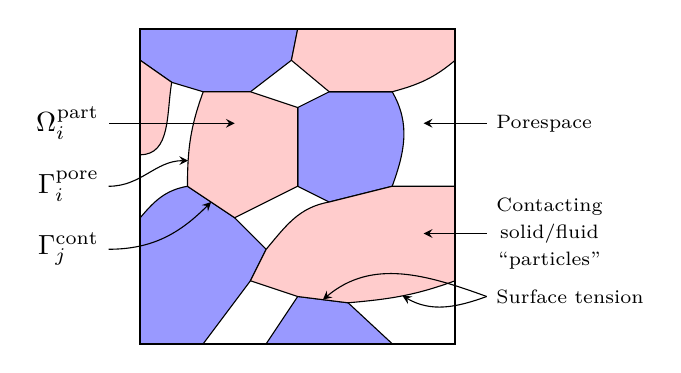
\begin{tikzpicture}[>=stealth,scale=4]
  \coordinate (A) at (0.35,0.2);
  \coordinate (B) at (0.4,0.3);
  \coordinate (C) at (0.3,0.4);
  \coordinate (D) at (0.15,0.5);
  \coordinate (E) at (0.66,0.13);
  \coordinate (F) at (0.6,0.45);
  \coordinate (G) at (0.8,0.5);
  \coordinate (H) at (0.5,0.5);
  \coordinate (I) at (0.5,0.75);
  \coordinate (J) at (0.6,0.8);
  \coordinate (K) at (0.8,0.8);
  \coordinate (L) at (0.35,0.8);
  \coordinate (M) at (0.5,1);
  \coordinate (N) at (0,0.9);
  \coordinate (O) at (0.1,0.83);
  \coordinate (P) at (0.5,0.15);
  \coordinate (Q) at (0.48,0.9);
  \coordinate (R) at (0.2,0.8);
  
  % Region 1 particles 
  \draw[fill=blue!40] 
  (0,0) -- (0.2,0) -- (A) -- (B) -- (C) -- (D) to[out=190,in=50] (0,0.4) -- cycle %A
  (0.4,0) -- (P) -- (E) -- (0.8,0) -- cycle %B
  (F) -- (G) to[out=70,in=-60] (K) -- (J) -- (I) -- (H) -- cycle %C
  (M) -- (Q) -- (L) -- (R) -- (O) -- (N) -- (0,1) -- cycle %D
  ;

  % Region 2 particles
  \draw[fill=red!20]
  (0,0.6) to[out=0,in=-100] (O) -- (N) -- cycle %E
  (D) to[out=90,in=-110] coordinate[near start] (surf3) (R) -- (L) -- (I) -- (H) -- (C) -- (D) coordinate[midway] (surf4) %F
  (M) -- (Q) -- (J) -- (K) to[out=15,in=-140] (1,0.9) -- (1,1) -- cycle %G
  (1,0.2) to[out=-160,in=5] coordinate[midway] (surf1) (E) -- (P) coordinate[midway] (surf2) -- (A) -- (B) to[out=50,in=-170] (F) -- (G) -- (1,0.5) -- cycle %H
  ;

  \draw[thick] (0,0) rectangle (1,1);

  % Annotations
  \draw[<-] (0.9,0.7) -- (1.1,0.7) node[right,font=\scriptsize] {Porespace};
  \draw[<-] (0.9,0.35) -- (1.1,0.35) node[right,font=\scriptsize] {\shortstack{Contacting\\solid/fluid\\``particles''}};
  \draw[<-] (surf1) to[out=-30,in=-160] (1.1,0.15) node[right,font=\scriptsize] {Surface tension};
  \draw[<-] (surf2) to[out=40,in=160] (1.1,0.15); % extra arrow
  \draw[<-] (surf3) to[out=180,in=0] (-0.1,0.5) node[left] {$\Gamma_i^{\mathrm{pore}}$};
  \draw[<-] (surf4) to[out=-135,in=0] (-0.1,0.3) node[left] {$\Gamma_j^{\mathrm{cont}}$};
  \draw[<-] (0.3,0.7) to[out=180,in=0] (-0.1,0.7) node[left] {$\Omega_i^{\mathrm{part}}$};
\end{tikzpicture}
    \caption{Microstructure of porous particulate material with sintering particles in contact. The sintering body is subjected to Dirichlet and Neumann boundary conditions on the external boundary.}
    \label{fig:micro}
\end{figure}
%-----------------------------------------------------------------------------


\subsection{Surface tension}

The ``surface tension'' along particle/particle and particle/pore interfaces (the latter denoted pore boundaries) is considered to be the sole ``driving force'' of the sintering process, and it is defined in terms of a ``surface tension force'' acting in the tangent plane of the surface. In the simplest (and most common) case of isotropic surface tension, this traction is characterized by the constant surface-specific surface energy $\gamma_\surf$ in the current configuration as the single material parameter. Although we adopt this simplified model below in the numerical results, it is possible to consider the more general situation of anisotropic ``surface stress'' that may also depend on the surface deformation via a suitable constitutive assumption, cf. \cite{Steinmann2008:boundaryenergies}.

As shown in, e.g. \textsc{Öhman et al.} \cite{OhmanRunLar2011}, it is possible to represent the surface tension force by an equivalent surface traction, henceforth denoted $\ta{t}_\fluct$, acting on the surface (or interface). In the presently assumed case of isotropic surface tension, $\ta{t}_\fluct$ is directed in the normal direction to the surface and is given as
%-----------------------------------------------------------------
\begin{equation}
    \ta{t}_\surf\defeq -\kappa\gamma_\surf\ta{n}
\label{eq103aKR}
\end{equation}
%------------------------------------------------------------------
where $\kappa\defeq\ta{n}\cdot\hat{\diff}$ is the curvature. Here, $\ta{n}$ is taken positive outwards from a convex surface, whereas $\hat\diff \defeq \diff - (\diff\cdot\ta{n})\ta{n}$ is the surface gradient operator.

%The smooth space-curved surface segment $\Gamma$, as shown in \figref{fig:surfacestress}, is considered as a ``thin shell'' acted upon by the tractions $\ta{t}^+$ and $\ta{t}^-$ on the upper and lower sides. These tractions are part of the final solution in the case $\Gamma$ is the contact interface of two bodies (solid or fluid) with different material properties. When $\Gamma$ is an outer surface, then $\ta{t}^+$ represents a prescribed loading (or reaction from prescribed displacement), whereas $-\ta{t}^-$ is the traction acting on the material just below the surface. In addition, the ``surface tension force'' $\hat{\ta t}$ acts in the tangent plane of the thin shell. Equilibrium is expressed as
%%-----------------------------------------------------------------
%\begin{equation}
%    \int_{\Gamma} \left[\ta{t}^+ + \ta{t}^-\right] \dif a = \int_{\partial\Gamma} \hat{\ta t} \dif l = \ta{0}
%\label{eq101KR}
%\end{equation}
%%------------------------------------------------------------------
%Upon introducing the ``surface stress'' tensor $\hat{\ts\sigma}$ (with components only in the tangent plane), such that $\hat{\ta t}=\hat{\ts\sigma}\cdot\ta{m}$ and $\hat{\ts\sigma}\cdot\ta{n}=\ta{0}$, we may use the surface divergence theorem for a smooth surface segment to rephrase the curve integral in \eqref{eq101KR} as
%%-----------------------------------------------------------------
%\begin{equation}
%    \int_{\partial\Gamma} \hat{\ts\sigma}\cdot\ta{m} \dif l = \int_{\Gamma} \hat{\ts\sigma}\cdot\hat{\diff} \dif a + \int_{\Gamma} \kappa\hat{\ts\sigma}\cdot\ta{n} \dif a = \int_{\Gamma} \hat{\ts\sigma}\cdot\hat{\diff} \dif a
%\label{eq102KR}
%\end{equation}
%%------------------------------------------------------------------
%Here, $\hat\diff \defeq \diff - \ta{n}\nabla_n$ is the surface gradient operator and $\kappa\defeq\ta{n}\cdot\hat{\diff}$ is the curvature and $\ta{n}\defeq\ta{n}^+$ is taken positive outwards from a convex surface. Combining \eqref{eq101KR} and \eqref{eq102KR} and localizing the result for any arbitrary choice of $\Gamma$, we obtain the strong format of traction equilibrium as follows:
%%-----------------------------------------------------------------
%\begin{equation}
%    \ta{t}^+ + \ta{t}^- + \ta{t}_\surf = \ta{0} \quad \mbox{on} \,\, \Gamma \quad \mbox{with } \ta{t}_\surf \defeq \hat{\ts\sigma}\cdot\hat{\diff}
%\label{eq103KR}
%\end{equation}
%%------------------------------------------------------------------
%where $\ta{t}_\surf$ is the ``surface tension traction''. Since it can be shown that $\ta{t}_\surf$ will depend on the (local) curvature, it is well-defined only when $\Gamma$ is sufficiently smooth
%
%Special case: Isotropic surface tension:
%
%Consider the special case that the surface tension is isotropic and homogeneous in the spatial format, i.e. $\hat{\ts\sigma}=\gamma_\surf\hat{\ts I}$, where $\gamma_\surf$ is a constant parameter and $\hat{\ts I} \defeq \ts{I} - \ta{n}\outerp\ta{n}$ is the surface identity tensor. Using the identity $\hat{\ts I}\cdot\hat{\diff}=-\kappa\ta{n}$, we then obtain
%%-----------------------------------------------------------------
%\begin{equation}
%    \sum_i \gamma_{\surf,i}\ta{m}_i = \ta{0} \quad \mbox{on} \,\, \mathcal{C}
%\label{eq104aKR}
%\end{equation}
%%------------------------------------------------------------------


\subsection{Incompressible viscous flow of the Stokes' type}

We shall adopt a model for the subscale deformation within the solid particles undergoing the time-dependent sintering process. The model is simplified in the sense that elastic deformation is neglected a priori. It is then possible to consider a viscoplastic (fluid-like) material with intrinsic incompressibility (within the particles). Such incompressibility is expressed as $d_\vol\defeq\ta{v}\cdot\ts{\nabla}=0$ and, hence, $\ts{d}_\dev=\ts{d}$. An isotropic and associated viscoplastic flow rule of the classical Perzyna type is the proposed in the following restricted fashion:
%-----------------------------------------------------------------
\begin{equation}
    \ts{d}=\ts{d}_\dev = \frac{1}{2\mu}\ts{\sigma}_\dev + \ts{d}_\dev^\pl(\ts{\sigma}_\dev), \quad
    \ts{d}_\dev^\pl = \frac{1}{t_*}\eta\left(\Phi\left(\sigma_\eqv\right)\right)\od{\Phi}{\ts\sigma}
\label{eq201}
\end{equation}
%------------------------------------------------------------------
where $t_*$ is the relaxation time, $\eta(\Phi)$ is an overstress function, $\Phi(\sigma_\eqv)$ is the quasistatic yield function and $\sigma_\eqv=\sqrt{\frac{3}{2}}|\ts{\sigma}_\dev|$ is the equivalent stress. Upon introducing the abbreviated notation $k=\frac{\eta}{t_*}\od{\Phi}{\sigma_\eqv}$, we may solve for $\sigma_\eqv$ in terms of the equivalent rate of deformation $d_\eqv\defeq\sqrt{\frac{2}{3}}|\ts{d}_\dev|$ from the equation
%-----------------------------------------------------------------
\begin{equation}
    \frac{1}{3\mu}\sigma_\eqv + k\left(\sigma_\eqv\right) = d_\eqv
\label{eq202}
\end{equation}
%------------------------------------------------------------------
and we, finally, obtain the ``Newtonian-like'' constitutive relation
%-----------------------------------------------------------------
\begin{equation}
    \ts{\sigma}_\dev(\ts{d}) = 2\tilde{\mu}\ts{d}_\dev, \quad
    \tilde{\mu}\defeq \frac{\sigma_\eqv}{3d_\eqv}
    %\frac{\mu}{1+\frac{3\mu k\left(\sigma_\eqv\left(d_\eqv\right)\right)}{\sigma_\eqv\left(d_\eqv\right)}}
\label{eq203}
\end{equation}
%------------------------------------------------------------------

The corresponding tangent stiffness $\tf{E}_{\tang,\dev}$ in the relation $\dif\ts{\sigma}_\dev=\tf{E}_{\tang,\dev}\dprod\dif\ts{d}$ (representing the linearization of the subscale constitutive problem), is given as follows:
%------------------------------------------------------------------
\begin{align}
 \tf E_{\tang,\dev} &= 2\tilde{\mu} \tf I_\dev + \frac{4}{9 d_\eqv^2} \left[ d_\eqv \left[ \frac{1}{3\mu} + k' \right]^{-1} - \sigma_\eqv \right] \ts d_\dev \outerp\ts d_\dev
 %\intertext{with}
 ,\quad k' = \frac{1}{t_*}\left[\eta \frac{\mathrm{d}^2\;\Phi}{\dif\sigma_\eqv^2} + \od{\eta}{\Phi}\left[\od{\Phi}{\sigma_\eqv}\right]^2\right].
\end{align}
%------------------------------------------------------------------

In the absence of acceleration, the balance equations for the quasi-static motion of the viscoplastic particles can be established in the spatial setting as follows:
%-----------------------------------------------------------------
\begin{align}
    -\ts{\sigma}\cdot\diff & = \ts{0} \quad \mbox{ in }\,\Omega
\label{eq204a}
\\
    \ta{v}\cdot\diff & = 0 \quad \mbox{ in }\,\Omega
\label{eq204b}
\end{align}
%------------------------------------------------------------------
where $\ts{\sigma}(\ts{d})=\ts{\sigma}_\dev(\ts{d})-p\ts{I}$ is the total Cauchy stress, $p$ is the pressure (Lagrangian multiplier corresponding to the incompressibility constraint), and
where $\diff$ denotes the spatial gradient.

In order to establish the weak format of \eqref{eq204a} and \eqref{eq204b} for a sintering body, we adopt standard Dirichlet and Neumann boundary conditions on the (external) boundary parts $\Gamma^\external_\Dirichlet$ and $\Gamma^\external_\Neumann$, respectively. In particular, prescribed tractions, $\bar{\ta t}_\prescribed$, act on $\Gamma^\external_\Neumann$. Referring to \figref{fig:micro}, we identify smooth pore surfaces $\Gamma^\pore=\cup_i\Gamma^\pore_i$ and smooth contact surfaces $\Gamma^\contact=\cup_j\Gamma^\contact_j$. These surfaces, that are internal to the microstructure, are collectively denoted $\Gamma^\internal=\Gamma^\pore\cup\Gamma^\contact$. It can then be shown that the space-variational forms of \eqref{eq204a} and \eqref{eq204b} read:
%Boundary conditions are given on the Dirichlet and Neumann parts of the boundary $\partial\Omega_\Box$ of the ``flow domain'' $\Omega_\Box$, denoted $\partial\Omega_{\Box, \Dirichlet}$ and $\partial\Omega_{\Box, \Neumann}$, respectively. Firstly, it is clear that $\Gamma_\Box^{\rm f}\subseteq\partial\Omega_{\Box, \Neumann}$, i.e. the free boundary is always a Neumann boundary. The appropriate boundary condition on $\Gamma_\Box^{\rm f}$ will be defined below. Secondly, we note that $\bar{\Gamma}_\Box\nsubseteq\partial\Omega_{\Box,\Neumann}$ in the case of Dirichlet boundary conditions, while $\bar{\Gamma}_\Box\subseteq\partial\Omega_{\Box,\Neumann}$ in the case of Neumann boundary conditions. With the issue of the appropriate choice of boundary conditions left unsettled for the moment, we merely note that the space-variational forms of \eqref{eq204a} and \eqref{eq204b} read:
%-----------------------------------------------------------------
\begin{align}
    \int_{\Omega} \ts{\sigma}\dprod\delta \ts{d} \dif v
    & =
    \int_{\Gamma^\internal} \ta{t}_\surf \cdot \delta\ta{v} \dif a
%    - \int_{\Gamma^\internal} \hat{\ts\sigma}\dprod\left[\delta\ta{v}\outerp\hat{\diff}\right] \dif a
    + \int_{\Gamma^\external_\Neumann} \bar{\ta t}_\prescribed\cdot\delta \ta{v} \dif a
\label{eq205a} \\
    \int_{\Omega} \left[\ta{v}\cdot\diff\right] \delta p \dif v
    & =  0
\label{eq205b}
\end{align}
%------------------------------------------------------------------
for suitable test functions $\delta\ta{v}$ and $\delta p$ that satisfy the appropriate regularity requirements (not further elaborated in this paper). Here it was used that $\delta\ta{v}=\ta{0}$ on $\Gamma^\external_\Dirichlet$.

\textbf{Remark}: In the special case of isotropic surface tension (not necessarily state-independent or homogeneous), the operational format of \eqref{eq205a} is obtained by using the more explicit expression for the integral that represents ``surface tension loading'':
%-----------------------------------------------------------------
\begin{equation}
    \int_{\Gamma^\internal} \ta{t}_\surf \cdot \delta\ta{v} \dif a =
    \int_{\Gamma^\internal} \gamma_\surf\left[\delta\ta{v}\cdot\hat{\diff}\right] \dif a
\label{eq206}
\end{equation}
%------------------------------------------------------------------
where the surface divergence theorem was used for any smooth pore surface segment $\Gamma^\pore_i$. $\Box$

\subsection{Representative Volume Element \textbf{UPDATE}}

An appropriately chosen RVE is assumed to occupy the bulk volume $\Omega_\Box(t)$ with side length $L_\Box(t)\defeq(|\Omega_\Box(t)|)^{1/\NDIM}$, where $\NDIM$ is the problem dimension (2 or 3). The RVE must obviously contain a sufficient number of particles and pores to qualify as ``representative'' in the classical sense; however, in order to simplify the subsequent conceptual discussion and ``pave the way'' for the subsequent homogenization, we shall henceforth restrict the analysis to 2D, and we consider a simple arrangement of particles within the RVE. In the very simplest case that the RVE consists of one single ``unit cell'' containing a single contiguous pore in the 2D-projection.

The current ``bulk'' domain of the RVE at a time $t>0$ contains the particles and the pore space, $\Omega_\Box(t)=\Omega^\particle_\Box(t)\cup\Omega_\Box^\pore(t)$, where $\Omega_\Box^\pore(t)$ is the domain currently occupied by the pore, whereas $\Omega_\Box^\particle(t)$ is occupied by the particles. This is shown schematically in \figref{fig:4particle_rve_b}.
%\footnote{Henceforth, when the time argument is dropped, e.g. $\Omega_\Box$, the current configuration is referred to.}.
The external boundary of the RVE is $\partial\Omega_\Box(t)\defeq\Gamma_\Box(t)$. The initial configuration of the particles within the RVE (before any deformation has taken place) is denoted $\Omega_\Box(0)$, as shown in \figref{fig:4particle_rve_a}. It is noted that in 2D, by assumption, the external boundary of the RVE always cuts through the particles and never through the pore space. The boundaries of the (closed) pore-space are collectively denoted $\Gamma_\Box^\pore(t)$. For simplicity (but without loosing generality of the formulation), we shall henceforth ignore contributions from interfaces between contacting particles. The boundary of the deforming particles currently contained in the RVE is then $\partial\Omega^\particle_\Box(t)=\Gamma_\Box(t)\cup\Gamma_\Box^\pore(t)$.
%-------------------------------------------------------------------------
\begin{figure}[th!]
    \centering
    \subfloat[$t = 0$]{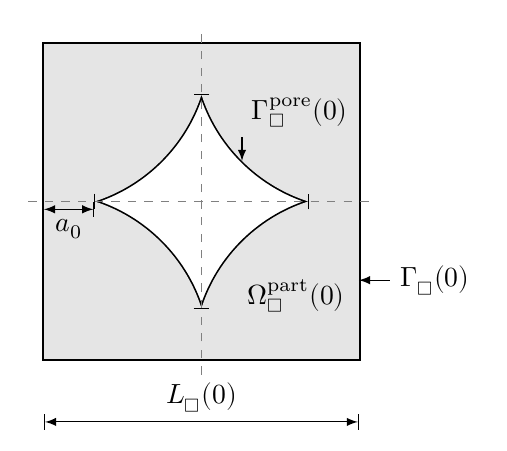
\begin{tikzpicture}[>=latex,scale=2] % Use this to scale the image. Text is always normal-size
  \def\particleradius{1.05} % Adjust this to change the contact size.
  \pgfmathsetmacro{\contactsize}{sqrt(\particleradius^2-1)} % Automatically calculated.
  \begin{scope}[very thick]
  	\draw[clip] (-1,-1) rectangle (1,1);
  	\draw[clip]
  		(-1,-1) circle (\particleradius)
 		( 1,-1) circle (\particleradius)
 		(-1, 1) circle (\particleradius)
   		( 1, 1) circle (\particleradius);
  	\fill[fill=black!10] (-1,-1) rectangle (1,1);
  \end{scope}
  % Markers
  \foreach \q in {0,90,180,270} { \draw[rotate=\q] (1-\contactsize,-0.05) -- +(0,0.1); }
  \draw[dashed,gray] (-1.1,0) -- (1.1,0) (0,-1.1) -- (0,1.1);
  % Annotations
  %\node[below] at (0,0) {$\Omega_\Box^p(0)$};
  \draw[|<->|] (-1,-1.4) -- (1,-1.4) node[midway,above] {$L_\Box(0)$};
  \draw[<->|] (-1,-0.05) -- +(\contactsize,0) node[midway,below] {$a_0$};
  \node at (0.6,-0.6) {$\Omega_\Box^{\mathrm{part}}(0)$};
  \draw[<-] (1,-0.5) -- +(0.2,0) node[right] {$\Gamma_\Box(0)$};
  \draw[<-] (1,1) ++(-135:\particleradius) -- +(0.00,0.15) node[above right] {$\Gamma_\Box^{\mathrm{pore}}(0)$};
  
  %\draw[use as bounding box] (-1.7,-1.5) rectangle (1.7,1.1);
  %\useasboundingbox (-1.7,-1.5) (1.7,1.1);
  % Transformation arrow (makes the picture very unaligned)
  %\draw[->] (1.5,0) to[out=45,in=-150] (2,0);% +(135:0.1) -- (2,0) -- +(-135:0.1);
\end{tikzpicture}
\label{fig:4particle_rve_a}}
    \subfloat[$t > 0$]{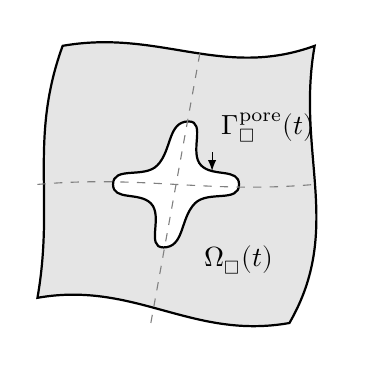
\begin{tikzpicture}[>=latex,scale=1.6] % Use this to scale the image. Text is always normal-size
  \def\particleradius{1.05} % Adjust this to change the contact size.
  \draw[thick,fill=black!10,even odd rule] (0.9,-1.1) 
  	to[out=190,in=10] (-1.1,-0.9)
  	to[out=80,in=-110] (-0.9,1.1)
  	to[out=10,in=-160] (1.1,1.1)
  	to[out=-100,in=60] (0.9,-1.1) -- cycle
  	(-0.1,-0.5) to[out=180,in=-45] (-0.2,-0.15) to[out=135,in=-90]
  	(-0.5,0)    to[out=90,in=-135] (-0.15,0.15)  to[out=45,in=-180]  
  	(0.1,0.5)   to[out=0,in=135]   (0.2,0.15)   to[out=-45,in=90] coordinate[near start] (GammaF)
  	(0.5,0)     to[out=-90,in=45]  (0.15,-0.15)  to[out=-135,in=0] (-0.1,-0.5) -- cycle;
  % Markers
  \draw[dashed,gray] (-1.1,0) to[out=5,in=-175] (1.1,0) (-0.2,-1.1) -- (0.2,1.1);
  % Annotations
  \node at (0.5,-0.6) {$\Omega_\Box(t)$};
  \draw[<-] (GammaF) -- +(0.00,0.15) node[above right] {$\Gamma_\Box^{\mathrm{pore}}(t)$};
\end{tikzpicture}\label{fig:4particle_rve_b}}
    \caption{(a) Initial configuration of RVE in 2D consisting of circular particles in a perfect square lattice. The contact ``points'' are flattened due to precompaction. (b) Deformed configuration (sketchy).}
    \label{fig:4particleRVE}
\end{figure}
%-----------------------------------------------------------------------------

\section{Macroscale problem}\label{sec:macro}

\subsection{Transition to macroscopic incompressibility}

In the paper by \textsc{Öhman et al.} \cite{OhmanRunLar2011} the macroscale format is restricted to the situation that the response is compressible. However, this format is inadequate and the algorithm breaks down when the macroscale response becomes incompressible, which situation is encountered when the porosity vanishes (locally). This is intuitively clear; however, it can be shown readily as follows:

Consider the RVE occupying the current domain $\Omega_\Box$, as shown in Figure \ref{fig:4particleRVE}, and consider the condition of intrinsic incompressibility, $\ta{v}\cdot\diff=0$ in $\Omega_\Box^\particle$, from which it follows that
%----------------------------------------------------------------------------
\begin{equation}
    \langle \ta{v}\cdot\diff \rangle_\Box  = 0
\label{eq230}
\end{equation}
%----------------------------------------------------------------------------
In standard fashion, the explicit part of the prolonged macroscale field, denoted $\ta{v}^\macro$, is assumed to vary only \emph{linearly} within the RVE, i.e.
%----------------------------------------------------------------------------
\begin{equation}
    \ta{v} = \ta{v}^\macro + \ta{v}^\fluct =
    \bar{\ts d} \cdot [\ta{x}-\bar{\ta{x}}] + \ta{v}^\fluct \mbox{ for }\ta{x}\in\Omega_\Box,
    \label{eq409}
\end{equation}
%----------------------------------------------------------------------------
where $\bar{\ts d}=\bar{\ts d}(\bar{\ta{x}})=\bar{\ts d}=\bar{\ts d}_\dev+\frac{1}{3}\bar{d}_\vol\ts{I}$ is the value of the macroscale rate-of-deformation tensor in the center of the RVE. Upon introducing this relation into \eqref{eq230}, we obtain directly (with $\bar{d}_\vol\defeq\ts{I}\dprod\bar{\ts d}=\bar{\ta v}\cdot\diff$) the identity
%----------------------------------------------------------------------------
\begin{equation}
    \bar{d}_\vol = - \frac{1}{1-\phi}\frac{1}{|\Omega_\Box|}\int_{\Gamma_\Box^\pore\cup\Gamma_\Box} \ta{v}^\fluct\cdot\ta{n} \dif a
    \label{eq410}
\end{equation}
%----------------------------------------------------------------------------
where $\phi\defeq 1-\frac{\Omega_\Box^\particle}{\Omega_\Box}$ is the (current) macroscopic porosity. The fluctuation field $\ta{v}^\fluct\{\bar{\ts d}\}$ is computed from the RVE-problem for given value of $\bar{\ts d}$. Now, let us consider the situation of Dirichlet\marginpar{other bc?} boundary conditions in the RVE-problem, $\ta{v}^\fluct=\ta{0}$, on (the exterior boundary) $\Gamma_\Box$ and the boundary integral in \eqref{eq410} reduces to $\Gamma_\Box^\pore$. When the porosity vanishes, then $\Gamma_\Box^\pore$ disappears and we obtain $\bar{d}_\vol = 0$, which is a ``pathological'' situation from the point of view of the macroscale format. It is noted that, from the moment incompressibility is a fact, it is possible to trace the isochoric macroscale flow only if a mixed variational format is employed in terms of $(\bar{\ta v},\bar{p})$, where $\bar{p}$ is the macroscale pressure (negative mean stress). This mixed format is derived next.


\subsection{Mixed format of the macroscale problem}

\subsubsection{Preliminaries}

Classical model-based homogenization is adopted upon introducing the volume-averaged virtual work equation in \eqref{eq205a} on the characteristic Representative Volume Element (RVE), as defined in Figure \ref{fig:4particleRVE}, and integrating on the entire macroscopic domain $\Omega(t)$. We may then express the homogenized internal virtual work as
%----------------------------------------------------------------------------------------------------
\begin{equation}
    a(\ta{v},p; \delta \ta{v}^\macro) \defeq
    \int_{\Omega} \left[
    a_\Box(\ta{v};\delta \ta{v}^\macro) + b_\Box(p, \delta \ta{v}^\macro) - l_\Box^\pore(\delta \ta{v}^\macro)
    \right] \dif \bar{v}
\label{eq402a}
\end{equation}
%-----------------------------------------------------------------------------------------------------
where we introduced the subscale variational forms\footnote{$\langle[\bullet]\rangle_\Box\defeq\frac{1}{|\Omega_\Box|}\int_{\Omega^\fluid_\Box}[\bullet] \, \dif v$ is the bulk volume average on the RVE of a quantity associated with particles in the domain $\Omega_\Box$.}
%----------------------------------------------------------------------------
\begin{align}
    a_\Box(\ta{v};\delta \ta{v})
    & \defeq
    \langle \ts{\sigma}_\dev(\ts{d}) \dprod \delta \ts{d} \rangle_\Box =
    \frac{1}{|\Omega_\Box|}\int_{\Omega^\fluid_\Box} \ts{\sigma}_\dev(\ts{d}) \dprod \left[\delta \ta{v}\outerp\diff\right]^\sym \dif v
\label{eq403a}
\\
    b_\Box(p, \ta{v})
    & \defeq
    - \langle p\,\ts{I}\dprod\ts{d} \rangle_\Box =
    - \langle p\,\ta{v}\cdot\diff \rangle_\Box =
    - \frac{1}{|\Omega_\Box|}\int_{\Omega^\fluid_\Box} p \left[\ta{v}\cdot\diff\right] \dif v
\label{eq403b}
\\
    l_\Box^\pore(\delta \ta{v})
    & \defeq
    \frac{1}{|\Omega_\Box|} \int_{\Gamma_\Box^\pore} \ta{t}_\surf \cdot \delta\ta{v} \dif a
\label{eq403c}
\end{align}
%----------------------------------------------------------------------------
for suitably chosen test velocity field $\delta\ta{v}$ such that $\delta\ts{d}\defeq\left(\delta\ta{v}\outerp\diff\right)^\sym$ is the corresponding rate-of-deformation tensor.

We next use the decomposition of the local velocity field within each RVE as represented in \eqref{eq409}, which may be inserted into \eqref{eq402a} to give
%%----------------------------------------------------------------------------
%\begin{eqnarray}
%    \ta{v}
%    & = &
%    \ta{v}^\macro + \ta{v}^\fluct = \ta{v}^\macro_\dev(\bar{\ts d}_\dev) +  \ta{v}^\macro_\vol(\bar{d}_\vol) + \ta{v}^\fluct
%    \nonumber \\
%    & = &
%    \bar{\ts d}_\dev \cdot [\ta{x}-\bar{\ta{x}}] + \bar{d}_\vol\ta{x}_\mean + \ta{v}^\fluct \mbox{ for }\ta{x}\in\Omega_\Box,
%    \quad \ta{x}_\mean\defeq\frac{1}{3}[\ta{x}-\bar{\ta{x}}]
%    \label{eq403d}
%\end{eqnarray}
%%----------------------------------------------------------------------------
%which gives the corresponding decomposition of $\ts{d}$ as follows:
%%----------------------------------------------------------------------------
%\begin{equation}
%    \ts{d} = (\ta{v}\outerp\diff)^\sym = \ts{d}^\macro_\dev + \ts{d}^\macro_\vol + \ts{d}^\fluct =
%    \bar{\ts d}_\dev + \frac{1}{3}\bar{d}_\vol\ts{I} + \ts{d}^\fluct \mbox{ for }\ta{x}\in\Omega_\Box,
%    \label{eq403e}
%\end{equation}
%%----------------------------------------------------------------------------
%Upon inserting the relations \eqref{eq403d}, \eqref{eq403e} into \eqref{eq402a}, we obtain the equation
%----------------------------------------------------------------------------
\begin{equation}
    a(\ta{v},p; \delta \ta{v}^\macro) =
    \int_\Omega
    \left[\bar{\ts\sigma}_{\dev} \dprod \delta\bar{\ts d}_\dev -
    \bar{p}\delta\bar{d}_\vol\right] \dif v =
    \int_\Omega
    \left[\bar{\ts\sigma}_{\dev} \dprod \left[\delta\bar{\ta v}\outerp\diff\right]^\sym_\dev -
    \bar{p}\left[\delta\bar{\ta v}\cdot\diff\right]\right]
    \dif v = 0
    \label{eq403f}
\end{equation}
%----------------------------------------------------------------------------
In \eqref{eq403f}, we introduced the deviatoric energy-conjugated macroscale stress tensor $\bar{\ts\sigma}_\dev$ and the macroscale pressure $\bar{p}$, which are deduced as follows: $\bar{\ts\sigma}_\dev\defeq\bar{\ts\sigma}+\bar{p}\ts{I}$, $\bar{p}\defeq-\frac{1}{3}\bar{\ts\sigma}\dprod\ts{I}$ with
%-----------------------------------------------------------------
\begin{equation}
    \bar{\ts\sigma} =
    \langle \ts{\sigma} \rangle_\Box - 
    \frac{1}{|\Omega_\Box|}\int_{\Gamma_\Box^\pore} \left[\ta{t}_\fluct\outerp[\ta{x}-\bar{\ta{x}}]\right]^\sym \dif a =
    \frac{1}{|\Omega_\Box|}\int_{\Gamma_\Box} \left[\ta{t}\outerp[\ta{x}-\bar{\ta{x}}]\right]^\sym \dif a
\end{equation}
%------------------------------------------------------------------

\subsubsection{Compressible macroscale response}

As long as the porosity is non-zero and macroscopic compressibility prevails, the straight-forward approach is to carry out homogenization to obtain the macroscale stress $\bar{\ts\sigma}$ as an implicit function of $\bar{\ts d}$ (with $\bar{d}_\vol\neq 0$), i.e. we may write this implicit relation as
%----------------------------------------------------------------------------
\begin{equation}
   \bar{\ts\sigma} = \bar{\ts\sigma}_\Box\{\bar{\ts d}\} = \bar{\ts\sigma}_\Box\{\bar{\ts d}_\dev +\frac13\bar{d}_\vol\ts I\}
\label{eq416a}
\end{equation}
%----------------------------------------------------------------------------
However, in order to obtain a unified formulation that holds also for the situation when the macroscale response becomes incompressible, it is desirable to introduce a mixed variational format in terms of $\bar{\ts d}_\dev=\left(\bar{\ta v}\outerp\diff\right)^\sym_\dev$ and $\bar{p}$ as the ``prolongation variables'' that are imposed as input to the RVE-problem in a nested macroscale-subscale algorithm. This is achieved as follows:

For given values of $\bar{\ts d}_\dev$ and $\bar{p}$, the corresponding value $\bar{d}_\vol$ can be computed from the condition
%----------------------------------------------------------------------------
\begin{equation}
    -\frac13 \ts I\dprod \bar{\ts\sigma}_\Box\{\bar{\ts d}_\dev +\frac13\bar{d}_\vol\ts I\} = \bar p
\label{eq416}
\end{equation}
%----------------------------------------------------------------------------
and the solution is expressed as the the implicit function $\bar{d}_{\Box,\vol}\{\bar{\ts d}_\dev,\bar{p}\}$. The deviatoric stress can then be computed as
%----------------------------------------------------------------------------
\begin{equation}
    \bar{\ts\sigma}_{\dev} = \bar{\ts\sigma}_{\Box,\dev}\{\bar{\ts d}_\dev,\bar p\} \defeq \bar{\ts\sigma}_\Box\{\bar{\ts d}_\dev + \frac13 \bar{d}_\vol^*\ts I\} + \bar{p}\ts{I}
\label{eq418}
\end{equation}
%----------------------------------------------------------------------------
Finally, for given $\bar{\ts d}_\dev$ and $\bar{p}$, we summarize the ``mixed'' relations
%----------------------------------------------------------------------------
\begin{align}
 \bar{\ts\sigma} & =  \bar{\ts\sigma}_{\Box,\dev}\{\bar{\ts d}_\dev,\bar p\} - \bar p\ts I
\label{eq418a}\\
 \bar{d}_\vol & =  \bar{d}_{\Box,\vol}\{\bar{\ts d}_\dev, \bar p\}
\label{eq418b}
\end{align}
%----------------------------------------------------------------------------

\subsubsection{Incompressible macroscale response}

When the porosity vanishes and the macroscale response becomes incompressible, then $\bar{p}$ becomes a Lagrange multiplier corresponding to the constraint condition $\bar{d}_{\vol} = 0$. In other words, the relations in \eqref{eq418a}, \eqref{eq418b} are still valid if we set $\bar{d}_{\Box,\vol}\{\bar{\ts d}_\dev,\bar p\} = 0$.

\subsubsection{Mixed variational format of the macroscale problem}

Using the expressions \eqref{eq418a} and \eqref{eq418b}, we are in the position to formulate the ``unified'' macroscale problem as follows: Find $(\bar{\ta v},\bar p) \in\bar{\set V}\times\bar{\set{P}}$ that solve
%----------------------------------------------------------------------------
\begin{align}
 \bar a\{\bar{\ta v},\bar p; \delta\bar{\ta v}\} - \bar b\{\bar p, \delta\bar{\ta v}\} &= 0   \quad \forall\; \delta\bar{\ta v} \in \bar{\set{V}}^0
 \label{eq411a}\\
 - \bar b\{\delta\bar p, \bar{\ta v}\} + \bar c\{\bar{\ta v}, \bar p; \delta\bar p\}&= 0   \quad \forall\; \delta\bar p \in \bar{\set{P}}
 \label{eq411b}
\end{align}
%----------------------------------------------------------------------------
where the pertinent variational forms are given as
%----------------------------------------------------------------------------
\begin{align}
 \bar a\{\bar{\ta v},\bar p; \delta\bar{\ta v}\} &\defeq \int_\Omega \bar{\ts\sigma}_{\Box,\dev}\{\left[\bar{\ta v}\outerp \diff\right]^\sym_\dev,\bar p\}\dprod \left[\delta\bar{\ta v}\outerp \diff\right]^\sym_\dev \dif V
 \label{eq412a}\\
 \bar b\{\bar p, \delta\bar{\ta v}\}             &\defeq \int_\Omega \bar p\left[\delta\bar{\ta v}\cdot\diff\right]\dif V
 \label{eq412b}\\
 \bar c\{\bar{\ta v}, \bar p; \delta\bar p\}     &\defeq \int_\Omega \bar d_{\Box,\vol}\{\left[\bar{\ta v}\outerp \diff\right]^\sym_\dev,\bar p\}\delta\bar p\dif V
 \label{eq412c}
\end{align}
%----------------------------------------------------------------------------
Newton iterations employ the algorithmic tangents
%----------------------------------------------------------------------------
\begin{align}
% \dif \bar{\ts\sigma}_{\dev} =
 \dif \bar{\ts\sigma}_{\Box,\dev} &= \bar{\tf E}_\ded \dprod \dif\bar{\ts d}_\dev + \bar{\ts E}_\dep \dif\bar{p}
 \label{eq413a} \\
% \dif \bar{d}_{\vol} =
 \dif \bar{d}_{\Box,\vol} &= \bar{\ts C}_\ded \dprod \dif \bar{\ts d}_\dev + \bar{C}_\dep \dif\bar{p}
 \label{eq413b}
\end{align}
%-----------------------------------------------------------------------------
such that the increments $\Delta\bar{\ta v}$ and $\Delta\bar{p}$ are obtained from the system
%----------------------------------------------------------------------------
\begin{align}
 \bar{a}'_v\{\bullet; \delta\bar{\ta v},\Delta\bar{\ta v}\} + \bar{a}'_p\{\bullet; \delta\bar{\ta v},\Delta\bar{p}\} - \bar{b}\{\Delta\bar p, \delta{\ta v}\}
	  &= -\bar{a}\{\bullet; \delta\bar{\ta v}\} + \bar{b}\{\bullet, \delta\bar{\ta v}\}
\quad &&\forall \delta\bar{\ta v}\in \bar{\set{V}}^0
 \label{eq414a}\\
- \bar{b}\{\delta\bar p, \Delta\bar{\ta v}\} + \bar{c}'_v\{\bullet; \delta\bar{p}, \Delta\bar{ \ta v}\} + \bar{c}'_p\{\bullet; \delta\bar{p},\Delta\bar{p}\}
	  &= \bar{b}\{\delta\bar{p},\bullet\} - \bar{c}\{\bullet;\delta\bar{p}\}
\quad &&\forall \delta\bar{p} \in \bar{\set{P}}
 \label{eq414b}
\end{align}
%----------------------------------------------------------------------------
where
%----------------------------------------------------------------------------
\begin{align}
 \bar{a}'_v\{\bullet; \delta\bar{\ta v},\Delta\bar{\ta v}\} &= \int_\Omega \left[\delta\bar{\ta v}\outerp\diff\right]^\sym_\dev \dprod \bar{\tf{E}}_\ded \dprod \left[\Delta\bar{\ta v}\outerp\diff\right]^\sym_\dev \dif V
 \label{eq415a}\\
 \bar{a}'_p\{\bullet; \delta\bar{\ta v},\Delta\bar{p}\}     &= \int_\Omega \left[\delta\bar{\ta v}\outerp\diff\right]^\sym_\dev \dprod \bar{\ts E}_\dep \,\Delta\bar{p} \dif V
 \label{eq415b}\\
 \bar{c}'_v\{\bullet; \delta\bar{p}, \Delta\bar{ \ta v}\}   &= \int_\Omega \delta\bar{p} \,\bar{\ts C}_\ded \dprod \left[\Delta\bar{\ta v}\outerp\diff\right]^\sym_\dev \dif V
 \label{eq415c}\\
 \bar{c}'_p\{\bullet; \delta\bar{p},\Delta\bar{p}\}         &= \int_\Omega \delta\bar{p} \,\bar{C}_\dep \Delta\bar p\dif V
 \label{eq415d}
\end{align}
%----------------------------------------------------------------------------
Once again we note that the problem in \eqref{eq411a}, \eqref{eq411b} does indeed represent both macroscopically compressible and incompressible states such that the transition is ``seamless''.
In the incompressible case, \eqref{eq411a}, \eqref{eq411b} can be replaced by the classical format
%----------------------------------------------------------------------------
\begin{align}
 \bar a\{\bar{\ta v},\bar p; \delta\bar{\ta v}\} - \bar b\{\bar p, \delta\bar{\ta v}\} &= 0   \quad \forall\; \delta\bar{\ta v} \in \bar{\set{V}}^0
 \label{eq420a}\\
 - \bar b\{\delta\bar p, \bar{\ta v}\} &= 0   \quad \forall\; \delta\bar p \in \bar{\set{P}}
 \label{eq420b}
\end{align}
%----------------------------------------------------------------------------
However, \eqref{eq411a}, \eqref{eq411b} is retained as the operational formulation in practice.

%The expression in \eqref{eq409} may conveniently be rewritten as
%----------------------------------------------------------------------------
%\begin{equation}
%    \ta{v}^\macro = \bar{\ts d} \cdot [{\ta x}-\bar{\ta x}] =
%    \sum_{i,j=1}^{\NDIM} \hat{\ta{v}}^{\macro(ij)} \bar{d}_{ij}
%    \label{eq409a}
%\end{equation}
%%----------------------------------------------------------------------------
%in terms of the ``unit velocity fields'' $\hat{\ta{v}}^{\macro(ij)}$ that are given as
%%----------------------------------------------------------------------------
%\begin{equation}
%    \hat{\ta{v}}^{\macro(ij)} \defeq \bee ij \cdot [{\bi x}-\bar{\bi x}] =
%    {\bi e}_i \left[x_j-\bar{x}_j\right]
%    \label{eq409b}
%\end{equation}
%%----------------------------------------------------------------------------
%The corresponding ``unit rate-of-deformation'' fields are given as
%$\hat{\ts{d}}^{\macro(ij)}\defeq(\hat{\ta{v}}^{\macro(ij)}\outerp\diff)^\sym=\left({\bi e}_{i}\outerp{\bi e}_{j}\right)^\sym$.
%
%From \eqref{eq402a} and \eqref{eq409a} we now obtain that $a(z;\delta\ta{v}^\macro)$ can be expressed as
%%----------------------------------------------------------------------------------------------------
%\begin{eqnarray}
%    a(z; \delta \ta{v}^\macro) & = &
%    \int_{\Omega} \sum_{i,j=1}^{\NDIM} \left[
%    a_\Box(\ta{v};\hbi{v}^{\macro(ij)}) + b_\Box(p, \hbi{v}^{\macro(ij)}) - l_\Box(\hbi{v}^{\macro(ij)})
%    \right] \delta \bar{d}_{ij}  \dif\bar{v}
%\label{eq409c}
%\end{eqnarray}
%%-----------------------------------------------------------------------------------------------------
%%Upon introducing \eqref{eq409} into \eqref{eq408}, we obtain the macroscale internal virtual work (space-variational) formulation
%Upon noting the definitions in \eqref{eq403a} to \eqref{eq403c}, we obtain the macroscale internal virtual work (space-variational) formulation
%%-----------------------------------------------------------------
%\begin{equation}
%    a(z; \delta \ta{v}^\macro) = \bar{a}\{\bar{\ta v}; \delta \bar{\ta v}\} \defeq
%    \int_{\Omega} \bar{\ts\sigma}\{\bar{\ts d}\} \dprod \delta \bar{\ts d} \dif\bar{v}
%\label{eq410}
%\end{equation}
%%------------------------------------------------------------------
%\textbf{Show this by using surface divergence thm etc. Introduce porosity $\Phi$?}
%
%
%Hence, the macroscale problem can be written as the residual equation
%%-----------------------------------------------------------------
%\begin{equation}
%    \bar{R}\{\bar{\ta v}; \delta \bar{\ta v}\} \defeq -\bar{a}\{\bar{\ta v}; \delta \bar{\ta v}\} = 0, \quad
%    \forall \delta\bar{\ta v}\in\bar{\set{V}}
%\label{eq410a}
%\end{equation}
%%------------------------------------------------------------------
%\textbf{Remark}: As to the proper relation between $\bar{\ts d}$ and the local field $\ts{d}$, we note that
%%-----------------------------------------------------------------
%\begin{eqnarray}
%\bar{\ts d}
%& = &
%\langle \ts{d} \rangle_\Box -
%\frac{1}{|\Omega_\Box|}\int_{\Gamma_\Box^\pore} (\ta{v}\outerp\ta{n})^\sym \dif a
%\nonumber \\
%& = &
%\frac{1}{|\Omega_\Box|}\int_{\Gamma_\Box} (\ta{v}\outerp\ta{n})^\sym \dif a
%\label{eq411b}
%\end{eqnarray}
%%-----------------------------------------------------------------
%This result is obtained under the assumptions that (i) the subscale velocity field is defined also within the pore space and is continuous along $\Gamma_\Box^\pore$, (ii) the bulk average of the fluctuation part of $\ts{d}$ vanishes, i.e. $\int_{\Omega_\Box}\left[\ts{d}-\ts{d}^\macro\right] \dif v = 0$. $\Box$
%
%In order to solve \eqref{eq410a} by Newton iterations, we need the tangent form
%%----------------------------------------------------------------------------
%\begin{equation}
%    \bar{a}'\{\bar{\ta v}; \delta\bar{\ta v},\Delta\bar{\ta v}\}
%    \defeq
%    \int_{\Omega} \delta \bar{\ts d} \dprod \bar{\tf E}_\majorT \dprod \Delta \bar{\ts d} \dif\bar{v}
%\label{eq105}
%\end{equation}
%%----------------------------------------------------------------------------
%The appropriate macroscale algorithmic tangent
%stiffness tensor, $\bar{\tf E}_\majorT$, is obtained upon linearizing the
%relation $\bar{\ts\sigma}\{\bar{\ts d}\}$ as follows:
%%----------------------------------------------------------------------------
%\begin{equation}
%  \dif \bar{\ts\sigma}\{\bar{\ts d}\} = \bar{\tf E}_\majorT\{\bar{\ts d}\} \dprod \dif \bar{\ts d}
%\label{eq106}
%\end{equation}
%%----------------------------------------------------------------------------
%and it is computed by \emph{linearization} of the RVE-problem, which
%leads to a \emph{sensitivity} or \emph{tangent} problem. How to
%formulate and solve this sensitivity problem in practice depends
%strongly on the actual choice of prolongation condition (as will be
%discussed below). In particular, the specific variational setting
%for every type of prolongation condition is different.
%
\section{RVE-problem for given macroscale fields}\label{sec:rve_problem}


\subsection{Variational format -- Dirichlet boundary conditions}

The task is to obtain the homogenized response for prescribed values of $\bar{\ts d}_\dev$ and $\bar{p}$. The variables to be returned to the macroscale equilibrium equation are $\bar{\ts\sigma}_\dev=\bar{\ts\sigma}_{\Box,\dev}\{\bar{\ts d}_\dev,\bar{p}\}$ and $\bar{d}_\vol=\bar{d}_{\Box,\vol}\{\bar{\ts d}_\dev, \bar{p}\}$. Henceforth, we shall adopt Dirichlet boundary conditions on the local fluctuation part of the velocity field, $\ta{v}^\fluct$. We are lead to the following trial and test spaces:
%%-----------------------------------------------------------------
%\begin{equation}
%    \ta{v} = \bar{\ts d} \cdot [\ta{x}-\bar{\ta{x}}]\,\,\mbox{on}\,\,\Gamma_\Box
%\label{eq211}
%\end{equation}
%%------------------------------------------------------------------
%----------------------------------------------------------------------------
\begin{align}
    \set V_\Box^{(\Dirichlet)} &= \{\ta{v} \mbox{ sufficiently regular in } \Omega_\Box, \,\, \ta{v}=\ta{0}\,\,\mbox{on}\,\,\Gamma_\Box\}
\label{eq:rve_functions_v}\\
    \set{P}_\Box &= \{p\in L_2(\Omega_\Box)\}
\label{eq:rve_functions_p}
\end{align}
%----------------------------------------------------------------------------
The appropriate space-variational format of the RVE-problem can now be formulated as follows (a derivation is given in the Appendix): For given macroscale variables $\bar{\ts d}_\dev$ and $\bar{p}$,
find ($\bar{d}_\vol,p,\ta{v}^\fluct)\in\set{R}\times\set{V}_\Box^{(\Dirichlet)}\times\set{P}_\Box$ that solve the system
%----------------------------------------------------------------------------
\begin{align}
    \label{eq213a} & a_\Box(\ta{v}^\macro_\dev + \ta{v}^\fluct;\delta \ta{v}^\fluct) +  b_\Box(p,\delta\ta{v}^\fluct)
    && =
    l^\pore_\Box(\delta \ta{v}^\fluct)
    && \forall \delta \ta{v}^\fluct\in\set{V}_\Box^{(\Dirichlet)}
 \\
    \label{eq213b} & b_\Box(\delta p, \ta{v}^\macro_\vol(\bar{d}_\vol)+\ta{v}^\fluct)
    && =
    0
    && \forall \delta p\in\set{P}_\Box
\\
    \label{eq213c} & b_\Box(p,\ta{x}_\mean)\delta\bar{d}_\vol
    && =
    [\bar{p} - l_\Box^\pore(\ta{x}_\mean)]\delta\bar{d}_\vol
    && \forall \delta\bar{d}_\vol  \in \set{R}
\end{align}
%----------------------------------------------------------------------------
%where we made explicit use of the local decomposition (within a given RVE) $\ta{v}=\ta{v}^\macro(\bar{\ts d})+\ta{v}^\fluct$ in terms of the ``macroscale'' part\footnote{The functional dependence on $\bar{\ts d}$ is explicit in the relation $\ta{v}^\macro(\bar{\ts d})$, whereas it is implicit in the relation $\ta{v}\{\bar{\ts d}\}$ for the total velocity.}, $\ta{v}^\macro(\bar{\ts d})=\bar{\ts d}\cdot[\ta{x}-\bar{\ta{x}}]$ and the
%fluctuation part, $\ta{v}^\fluct$.
%%fluctuation part, $\ta{v}^\fluct$, in standard fashion, together with the space-variational forms
%%----------------------------------------------------------------------------
%\begin{eqnarray}
%    a_\Box(\ta{v};\delta \ta{v})
%    & \defeq &
%    \langle \ts{\sigma}_\dev(\ts{d}) \dprod \delta \ts{d} \rangle_\Box =
%    \frac{1}{|\bar{\Omega}_\Box|}\int_{\bar{\Omega}_\Box} \ts{\sigma}_\dev(\ts{d}) \dprod \left(\delta \ta{v}\outerp\diff\right)^\sym \dif v
%\label{eq214a}
%\\
%    b_\Box(p, \ta{v})
%    & \defeq &
%    - \langle p\,\ts{I}\dprod\ts{d} \rangle_\Box =
%    - \langle p\,\ta{v}\cdot\diff \rangle_\Box =
%    - \frac{1}{|\bar{\Omega}_\Box|}\int_{\bar{\Omega}_\Box} p\, \ta{v}\cdot\diff \dif v
%\label{eq214b}
%\\
%    l_\Box(\delta \ta{v})
%    & \defeq &
%   % \frac{1}{|\bar{\Omega}_\Box|}\int_{\Gamma_\Box^\particle} \ta{t}\cdot \delta \ta{v} \dif a =
%    \frac{1}{|\bar{\Omega}_\Box|}
%    \left[\sum_{\beta=1}^{M_\segment}\int_{\Gamma_{\Box,\beta}^\particle} \gamma_\fluct\, \delta\ta{v}\cdot\tilde\diff \dif a - \sum_{\alpha=1}^{M_\corner} \gamma_\fluct\, \delta\ta{v}\cdot\left[\bi{m}_\alpha^{+} + \bi{m}_\alpha^{-}\right]\right]
%\label{eq214c}
%\end{eqnarray}
%%----------------------------------------------------------------------------

It is noted that the ``macroscale'' part, $\ta{v}^\macro=\ta{v}^\macro_\dev+\ta{v}^\macro_\vol$, of $\ta{v}$ is decomposed into the deviatoric part that is directly computed from the macroscale problem \eqref{eq:vMdev}, whereas the volumetric part \eqref{eq:vMvol}
is computed from the RVE-problem and is thus implicitly dependent on the macroscale solution via $\bar{\ts d}_\dev\defeq[\bar{\ta v}\outerp\diff]^\sym_\dev$ and $\bar{p}$.
\begin{align}
 \label{eq:vMdev} \ta{v}^\macro_\dev &\defeq \bar{\ts d}_\dev\cdot[\ta{x}-\bar{\ta{x}}]\\
 \label{eq:vMvol} \ta{v}^\macro_\vol &\defeq \bar{d}_\vol\ta{x}_\mean,\quad \ta{x}_\mean \defeq \frac13[\ta x-\bar{\ta x}]
\end{align}

The output variables from the RVE-problem are $\bar{d}_\vol$, which is a direct part of the solution, whereas $\bar{\ts\sigma}_\dev$ is post-processed as discussed subsequently.

The RVE-problem \eqref{eq213a} to \eqref{eq213c} must be solved iteratively in practice due to the
subscale nonlinearities. To this end, we first rewrite the RVE-problem as the vanishing residuals
%----------------------------------------------------------------------------
\begin{equation}
\begin{array}{rcll}
    R_\Box^{\ta v}(\bar{d}_\vol,\ta{v}^\fluct,p; \delta \ta{v}^\fluct)
    & \defeq &
    l_\Box^\pore(\delta \ta{v}^\fluct) -
    a_\Box(\ta{v}^\macro_\dev+\ta{v}^\fluct;\delta \ta{v}^\fluct) -
    b_\Box(p,\delta\ta{v}^\fluct)
    \quad & \forall \delta \ta{v}^\fluct\in\set{V}_\Box^{(\Dirichlet)}
    \\
%\label{eq13a} \\
    R_\Box^\dep(\bar{d}_\vol,\ta{v}^\fluct; \delta p)
    & \defeq &
    -  b_\Box(\delta p,\ta{v}^\macro_\vol(\bar{d}_\vol)+\ta{v}^\fluct)
    \quad & \forall \delta p\in\set{P}_\Box
    \\
     R_\Box^\ded(p;\delta\bar{d}_\vol)
    & \defeq &
    [\bar{p} - l_\Box^\pore(\ta{x}_\mean)- b_\Box(p,\ta{x}_\mean)]\delta\bar{d}_\vol
    \quad & \forall \delta\bar{d}_\vol  \in \set{R}
\end{array}
\label{eq250b}
\end{equation}
%----------------------------------------------------------------------------
Newton's iteration method for finding the unknown variables
$\bar{d}_\vol, \ta{v}^\fluct$ and $p$ for given $\bar{\ts d}_\dev$ and $\bar{p}$ then becomes: For $k=1,2,\ldots,$ compute
%----------------------------------------------------------------------------
\begin{equation}
    \bar{d}_\vol^{(k+1)} = \bar{d}_\vol^{(k)} + \Delta \bar{d}_\vol, \quad
    {\ta{v}}^{\fluct(k+1)} = {\ta{v}}^{\fluct(k)} + \Delta {\ta{v}}^\fluct, \quad
    p^{(k+1)} = p^{(k)} + \Delta p
\label{eq251}
\end{equation}
%----------------------------------------------------------------------------
where the iterative updates $\Delta\bar{d}_\vol\in\set{R}, \Delta {\ta{v}}^\fluct\in{\set{V}}_\Box^{(\Dirichlet)}$ and $\Delta p \in{\set{P}}_\Box$ are solved from the tangent equations
%----------------------------------------------------------------------------
\begin{equation}
\begin{array}{rcll}
    (a_\Box)'(\ta v^\macro_\dev + \ta v^\fluct; \delta\ta{v}^\fluct,\Delta \ta{v}^\fluct)
    + b_\Box(\Delta p,\delta\ta{v}^\fluct)
    & = &
    R_\Box^{\ta v}(\bullet^{(k)}; \delta\ta{v}^\fluct)
    \quad & \forall \delta \ta{v}^\fluct\in\set{V}_\Box^{(\Dirichlet)}
    \\
%\label{eq252a} \\
    b_\Box(\delta p,\ta{v}^\macro_\vol(\Delta\bar{d}_\vol) + \Delta\ta{v}^\fluct)
    & = &
    R_\Box^\dep(\bullet^{(k)}; \delta p)
    \quad & \forall \delta p\in\set{P}_\Box
    \\
    b_\Box(\Delta p,\ta{x}_\mean)\delta\bar{d}_\vol
    & = &
    R_\Box^\ded(\bullet^{(k)}; \delta\bar{d}_\vol)
    \quad & \forall \delta\bar{d}_\vol  \in \set{R}
\end{array}
\label{eq252b}
\end{equation}
%----------------------------------------------------------------------------
until the residuals are sufficiently small. The tangent form $(a_\Box)'$
is given explicitly as\todo{check!}
%----------------------------------------------------------------------------
\begin{align}
    (a_\Box)'(\ta v^\macro_\dev + \ta v^\fluct; \delta \ta{v}^\fluct,\Delta{\ta{v}}^\fluct)
    & = 
    \left\langle \left[\delta\ta{v}\outerp\diff\right]^\sym \dprod \tf{E}_{\majorT,\dev}(\ta v^\macro_\dev + \ta v^\fluct) \dprod
    \left[\Delta\ta{v}^\fluct\outerp\diff\right]^\sym \right\rangle_\Box
\end{align}
%----------------------------------------------------------------------------
\textbf{Remark}: In the macroscopically incompressible case, we will obtain $\bar{d}_\vol=0$ as part of the solution of the RVE-problem. $\Box$

\subsection{Macroscale algorithmic tensors}

The algorithmic tensors $\bar{\tf{E}}_\ded, \bar{\ts E }_\dep, \bar{\ts C}_\ded$ and $\bar{C}_\dep$, needed in order to carry out macroscale Newton iterations, are obtained for
perturbations of the RVE-solution expressed in terms of perturbations of $\bar{\ts d}_\dev$ and $\bar{p}$.
We first note that for a symmetric, deviatoric tensors, we can write
\begin{align}
 \bar{\ts\sigma}_\dev &= \sum_i^{n_{\mathrm{B}}} \bar{\sigma}_{\dev,i} \ts E_i,\quad \bar{\sigma}_{\dev,i} = \bar{\ts\sigma}_\dev\dprod \ts E_i\\
 \bar{\ts d}_\dev &= \sum_i^{n_{\mathrm{B}}} \bar{d}_{\dev,i} \ts E_i,\quad  \bar{d}_{\dev,i} = \bar{\ts d}_\dev\dprod \ts E_i
\end{align}
for an orthonormal base $\ts E_i$, such that $\ts E_i \dprod \ts E_j = \delta_{ij} $.\\
\textbf{Remark}: For 3D $n_{\mathrm{B}} = 5$, and for 2D $n_{\mathrm{B}} = 2$.

It is then convenient to compute \emph{sensitivity fields}, corresponding to a unit variation of the macroscale variables $\bar{\ts d}_\dev$ and $\bar{p}$. Hence, we shall need to compute the differentials, $\dif\bar p$ and
%----------------------------------------------------------------------------
\begin{align}
    \dif\ta{v}
     = &
    \dif\ta{v}^\macro_\dev + \dif\ta{v}^\macro_\vol + \dif\ta{v}^\fluct.
\label{eq:dv}
%\nonumber \\
%     = &
%    \dif\ta{v}^\macro_\dev + (\ta{v}^\macro_\vol)'_d \{\ta{v}^\macro_\dev,\bar{p};\dif\ta{v}^\macro_\dev\} + (\ta{v}^\macro_\vol)'_p \{\ta{v}^\macro_\dev,\bar{p};\dif\bar{p}\}
%\nonumber\\
%    &
%    +(\ta{v}^\fluct)'_d\{\ta{v}^\macro_\dev,\bar{p};\dif\ta{v}^\macro_\dev\} + (\ta{v}^\fluct)'_p\{\ta{v}^\macro_\dev,\bar{p};\dif\bar{p}\}
%\nonumber \\
%    & = &
%    \dif\bar{\ts d}_\dev[\ta{x}-\bar{\ta{x}}] + (\bar{d}_\vol)'_d\{\bar{\ts d}_\dev,\bar{p};\dif\bar{\ts d}_\dev\}\ta{x}_\mean + (\bar{d}_\vol)'_p \{\bar{\ts d}_\dev,\bar{p};\dif\bar{p}\}\ta{x}_\mean +
%\nonumber\\
%    &&
%    (\ta{v}^\fluct)'_d\{\bar{\ts d}_\dev,\bar{p};\dif\bar{\ts d}_\dev\} + (\ta{v}^\fluct)'_p\{\bar{\ts d}_\dev,\bar{p};\dif\bar{p}\}
%\label{eq215a}
%\\
%    \dif p
%     = &
%    (p)'_d\{\ta{v}^\macro_\dev,\bar{p};\dif\ta{v}^\macro_\dev\} + (p)'_p\{\ta{v}^\macro_\dev,\bar{p};\dif\bar{p}\}
%\nonumber \\
%    & = &
%    (p)'_d\{\bar{\ts d}_\dev,\bar{p};\dif\bar{\ts d}_\dev\} + (p)'_p\{\bar{\ts d}_\dev,\bar{p};\dif\bar{p}\}
%\label{eq215b}
\end{align}
%----------------------------------------------------------------------------------
% whereby $(\ta{v}^\macro_\vol)'_d, (\ta{v}^\macro_\vol)'_p, (\ta{v}^\fluct)'_d, (\ta{v}^\fluct)'_d$ and $(p)'$ denote directional derivatives.
From \eqref{eq:vMdev} and \eqref{eq:vMvol} respectively we obtain
%----------------------------------------------------------------------------
\begin{align}
  \dif \ta{v}^{\macro}_\dev &= \sum_{i} \hat{\ta{v}}^{\macro(i)}_\dev \dif\bar{d}_{\dev,i}, \quad  \hat{\ta{v}}^{\macro(i)}_\dev = \ts E_i \cdot [\ta x - \bar{\ta x}]
    \label{eq216}\\
\dif\ta{v}^\macro_\vol &= \ta x_\mean \dif \bar{d}_\vol
\end{align}
%----------------------------------------------------------------------------
where $\hat{\ta{v}}^{\macro(i)}_\dev$ are the ``unit velocity fields''. 
In analogy with the definition of $\hat{\ta{v}}^{\macro(i)}_\dev$
in \eqref{eq216}, we introduce the ``unit fields'', or sensitivities, due to a unit perturbation of the components $\dif\bar{d}_{\dev,i}$ and of $\dif\bar{p}$, via the \emph{ansatz}
%----------------------------------------------------------------------
\begin{align}
    \dif\bar{d}_\vol &= \sum_i \hat{\bar{d}}_{\vol,\ded}^{(i)}\dif\bar{d}_{\dev,i} + \hat{\bar{d}}_{\vol,\dep} \dif \bar{p}
\\
    \dif\ta v^\fluct &= \sum_i \hat{\ta{v}}_{\ded}^{\fluct(i)}\dif\bar{d}_{\dev,i} + \hat{\ta v}_{\dep}^\fluct \dif \bar{p}
\\
    \dif p           &= \sum_i \hat{p}_{\ded}^{(i)}\dif\bar{d}_{\dev,i} + \hat{p}_{\dep} \dif \bar{p}
%\\
%     (\ta{v}^\macro_\vol)'_d
%     & = 
%     \sum_{i}\hat{\ta{v}}^{\macro(i)}_{\vol,\ded} \dif\bar{d}_{\dev,i}, \quad
%     \hat{\ta{v}}^{\macro(i)}_{\vol,\ded} = \hat{\bar{d}}^{(i)}_{\vol,\ded}\ta{x}_\mean
% \label{eq221a} \\
%     (\ta{v}^\macro_\vol)'_p
%     & = 
%     \hat{\ta{v}}^{\macro}_{\vol,\dep} \dif\bar{p}, \quad
%     \hat{\ta{v}}^{\macro}_{\vol,\dep} = \hat{\bar{d}}_{\vol,\dep}\ta{x}_\mean
% \label{eq221b} \\
%     (\ta{v}^\fluct)'_d
%     & = 
%     \sum_{i}\hat{\ta{v}}^{\fluct(i)}_\ded\dif\bar{d}_{\dev,i},
% \label{eq222a} \\
%     (\ta{v}^\fluct)'_p
%     & = 
%     \hat{\ta{v}}^{\fluct}_\dep\dif\bar{p},
% \label{eq222b} \\
%     (p)'_d
%     & = 
%     \sum_{i}\hat{p}^{(i)}_\ded\dif\bar{d}_{\dev,i},
% \label{eq223a} \\
%     (p)'_p
%     & = 
%     \hat{p}_\dep\dif\bar{p}
% \label{eq223b}
\end{align}
%-----------------------------------------------------------------
Upon using the identity $\bar{\ts\sigma}=\frac{1}{\Omega_\Box} \int_{\Gamma_\Box} \ts t \outerp [\ta x - \bar{\ta x}]\dif a$, we deduce
%---------------------------------------------------------------------------------------
\begin{align}
    \dif\bar{\sigma}_{\dev,i}
    & = 
    \dif\bar{\ts\sigma}\dprod \ts E_i 
    =
    \dif\left[\frac{1}{\Omega_\Box} \int_{\Gamma_\Box} \ts t \cdot \ts E_i \cdot [\ta x - \bar{\ta x}]\dif a\right]
    =
    %\left\langle \dif\ts{\sigma}_\dev\dprod\left(\bee ij\right)^\sym\right\rangle_\Box=
    %\left\langle \dif\ts{\sigma}_\dev\dprod\hat{\ts{d}}^{\macro(ij)}_\dev\right\rangle_\Box=
    %\dif\left[\left\langle \ts{\sigma}_\dev \dprod \hat{\ts{d}}^{\macro(ij)}_\dev \right\rangle_\Box\right]
    %\nonumber \\
    %& = 
    -\dif\left[R_\Box^{\ts v}(\bullet;\hat{\ts v}_\dev^{\macro(i)})\right]
\nonumber\\
    &=
    \dif\left[a_\Box(\bullet; \hat{\ta{v}}^{\macro(i)}_\dev)\right] + \dif\left[b_\Box(\bullet; \hat{\ta{v}}^{\macro(i)}_\dev)\right] + \dif\left[l_\Box^\pore(\hat{\ta{v}}^{\macro(i)}_\dev)\right] = (a_\Box)'(\bullet; \hat{\ta{v}}^{\macro(i)}_\dev,\dif\ta{v})
    \nonumber \\
    & = 
    \underbrace{(a_\Box)'(\bullet;\hat{\ta{v}}^{\macro(i)}_\dev,\hat{\ta{v}}^{\macro(j)}_\dev +
    \hat{\ta{v}}^{\fluct(j)}_\ded)}_{\displaystyle \pd{\bar{\sigma}_{\dev,i}}{\bar{d}_{\dev,j}}}
    \dif\bar{d}_{\dev,j}
% Second term
    + \underbrace{(a_\Box)'(\bullet;\hat{\ta{v}}^{\macro(i)}_\dev, \hat{\ta{v}}^{\fluct}_\dep)}_{\displaystyle \pd{\bar{\sigma}_{\dev,i} }{ \bar{p} } }
    \dif\bar{p}.
    \label{eq219}
\end{align}
where we used that $b_\Box(\bullet;\hat{\ta v}_\dev^{\macro(i)}) = 0$ and $\dif\left[l_\Box^\pore\right(\hat{\ta v}^{\macro(i)}_\dev)] = 0$.
The full tensor form can be obtained from
\begin{align}
 \dif\bar{\ts\sigma}_\dev 
	&= \sum_i \ts E_i \dif\bar{\sigma}_{\dev,i}
	= \sum_{i,j} \ts E_i \pd{\bar{\sigma}_{\dev,i}}{\bar{d}_{\dev,j}} \dif\bar{d}_{\dev,j} + \sum_i \ts E_i \pd{\bar{\sigma}_{\dev,i}}{\bar{p}}\dif\bar{p}
\nonumber\\
	&= \sum_{i,j} \ts E_i \pd{\bar{\sigma}_{\dev,i}}{\bar{d}_{\dev,j}} [\ts E_j \dprod \dif\bar{\ts d}_{\dev}] + \sum_i \ts E_i \pd{\bar{\sigma}_{\dev,i}}{\bar{p}}\dif\bar{p}
\nonumber\\
    &= \underbrace{\left[\sum_{i,j} \pd{\bar{\sigma}_{\dev,i}}{\bar{d}_{\dev,j}} \ts E_i \outerp \ts E_j\right]}_{\displaystyle\bar{\tf E}_\ded} \dprod \dif\bar{\ts d}_{\dev}
	  + \underbrace{\sum_i \ts E_i \pd{\bar{\sigma}_{\dev,i}}{\bar{p}}}_{\displaystyle\bar{\ts E}_\dep}\dif\bar{p}
\end{align}
%------------------------------------------------------------------------------------
We also obtain trivially the relation
%---------------------------------------------------------------------------------------
\begin{align}
    \dif\bar{d}_\vol
    & = \sum_{i}\hat{\bar{d}}^{(i)}_{\vol,\ded}\dif\bar{d}_{\dev,i} + \hat{\bar{d}}_{\vol,\dep}\dif\bar{p}
      = \underbrace{\left[\sum_{i}\hat{\bar{d}}^{(i)}_{\vol,\ded} \ts E_i\right]}_{\displaystyle\bar{\ts C}_\ded} \dprod\dif\bar{\ts d}_{\dev} + \underbrace{\hat{\bar{d}}_{\vol,\dep}}_{\displaystyle\bar{C}_\dep}\dif\bar{p}
    \label{eq220}
\end{align}
%------------------------------------------------------------------------------------

In order to compute the pertinent sensitivities, we conclude that the state equations \eqref{eq213a} to \eqref{eq213c} must hold
for $\bar{\ts d}_\dev,\bar{p}$ as well as for a perturbed state $\bar{\ts d}_\dev+\dif\bar{\ts d}_\dev, \bar{p}+\dif\bar{p}$.
However, a given change $\dif\bar{\ts d}_\dev$ gives rise to a change, not only of $\dif\ta{v}^\macro_\dev$,
but also of $\dif\ta{v}^\macro_\vol$, $\dif\ta{v}^\fluct\in\set{V}_\Box^{(\Dirichlet)}$ and $\dif p\in\set{P}_\Box$.
Upon linearizing \eqref{eq213a} to \eqref{eq213c} , while using \eqref{eq:dv}, we obtain the appropriate tangent problem:
%----------------------------------------------------------------------------
\begin{align}
    &(a_\Box)'(\bullet;\delta\ta{v}^\fluct,\dif\ta{v}^\macro_\dev + \dif\ta{v}^\fluct) +
    b_\Box(\dif p,\delta\ta{v}^\fluct)
    && =
    0
    && \forall \delta \ta{v}^\fluct\in\set{V}_\Box^{(\Dirichlet)}
 \\
    &b_\Box(\delta p,\dif\ta{v}^\macro_\vol + \dif\ta{v}^\fluct)
    && =
    0
    && \forall \delta p\in\set{P}_\Box
\\
    &b_\Box(\dif p,\ta{x}_\mean)\delta\bar{d}_\vol
    && =
    \dif\bar{p}\delta\bar{d}_\vol
    && \forall \delta\bar{d}_\vol  \in \set{R}
\end{align}
%----------------------------------------------------------------------------
%%----------------------------------------------------------------------------
which must hold for any given $\dif\bar{\ts d}_\dev$ and $\dif\bar{p}$. We thus consider the cases ($\dif\bar{\ts d}_\dev\neq \ts{0}, \dif\bar{p}=0$) and ($\dif\bar{\ts d}_\dev=\ts{0}, \dif\bar{p}\neq 0$) in turn:

\begin{enumerate}
\item $\dif\bar{\ts d}_\dev = \ts E_i $ while $\dif\bar{p}=0$: For $i=1,\ldots,n_{\mathrm{B}}$, solve for the sensitivities $\hat{\bar{d}}^{(i)}_{\vol,\ded}$, $\hat{\ta{v}}^{\fluct(i)}_\ded$, and $\hat{p}^{(i)}_\ded$ from the system
%----------------------------------------------------------------------------
\begin{align}
    \label{eq233a} &
    (a_\Box)'(\bullet;\delta\ta{v}^\fluct,\hat{\ta{v}}^{\fluct(i)}_\ded) +
    b_\Box(\hat{p}^{(i)}_\ded,\delta\ta{v}^\fluct)
    && =
    - (a_\Box)'(\bullet;\delta\ta{v}^\fluct,\hat{\ta{v}}^{\macro(i)}_\dev)
    && \forall \delta \ta{v}^\fluct\in\set{V}_\Box^{(\Dirichlet)}
 \\
    \label{eq233b} &
    b_\Box(\delta p, \ta x_\mean \hat{\bar{d}}_{\vol,\ded}^{(i)} + \hat{\ta{v}}^{\fluct(i)}_\ded)
    && =
    0
    && \forall \delta p\in\set{P}_\Box
\\
    \label{eq233c} &
    b_\Box(\hat{p}^{(i)}_\ded,\ta{x}_\mean)\delta\bar{d}_\vol
    && =
    0
    && \forall \delta\bar{d}_\vol  \in \set{R}
\end{align}
%----------------------------------------------------------------------------

\item $\dif\bar{p} = 1$ while $\dif\bar{\ts d}_\dev=\ts{0}$: Solve for the sensitivities $\hat{\bar{d}}_{\vol,\dep}$, $\hat{\ta{v}}^{\fluct}_\dep$, and $\hat{p}_\dep$ from the system
%----------------------------------------------------------------------------
\begin{align}
    \label{eq243a} &
    (a_\Box)'(\bullet;\delta\ta{v}^\fluct,\ta x_\mean \hat{\bar{d}}_{\vol,\dep}+\hat{\ta{v}}^{\fluct}_\dep) +
    b_\Box(\hat{p}_\dep,\delta\ta{v}^\fluct)
    && =
    0
    && \forall \delta \ta{v}^\fluct\in\set{V}_\Box^{(\Dirichlet)}
 \\
    \label{eq243b} &
    b_\Box(\delta p,\ta x_\mean \hat{\bar{d}}_{\vol,\dep}+\hat{\ta{v}}^{\fluct}_\dep)
    && =
    0
    && \forall \delta p\in\set{P}_\Box
\\
    \label{eq243c} &
    b_\Box(\hat{p}_\dep,\ta{x}_\mean)\delta\bar{d}_\vol
    && =
    1\delta\bar{d}_\vol
    && \forall \delta\bar{d}_\vol  \in \set{R}
\end{align}
\end{enumerate}
%----------------------------------------------------------------------------
% We may express the source terms in \eqref{eq233a} and \eqref{eq233b} more explicitly as
% %\end{document}
% %----------------------------------------------------------------------------
% \begin{align}
%     (a_\Box)'(\bullet; \delta\ta{v},\hat{\ta{v}}^{\macro(i)}_\dev)
%     & = 
%     \langle \delta \ts{d} \dprod \tf{E}_{\majorT,\dev} \dprod \hat{\ts{d}}^{\macro(i)}_\dev \rangle_\Box
%     =
%     \langle \left(\left[\delta\ta{v}\outerp\diff\right]^\sym \dprod \tf{E}_{\majorT,\dev}\right)_{i} \rangle_\Box
% \label{eq263a}
% \\
%     b_\Box(\delta p,\hat{\ta{v}}^{\macro(i)}_\dev)
%     & = 
%     - \langle \delta p\,\ts{I}\dprod\hat{\ts{d}}^{\macro(i)}_\dev \rangle_\Box =
%     - \langle \delta p \rangle_\Box\, \delta_{ij}
% \nonumber
% \\
%     & = 
% %    - \left[\frac{1}{|\Omega_\Box|}\int_{\Omega_\Box} \delta p\, \dif v\right] \delta_{kl} =
%     - \frac{1}{|\Omega_\Box|}\int_{\Gamma_\Box} \delta p\, n_i [x_j-\bar{x}_j] \dif a
% \label{eq263b}
% \end{align}
% %----------------------------------------------------------------------------
% %
% %\subsubsection{Primal approach for computing the ATS tensor}
% 
% %%--------------------------------------------------------------------
% %\begin{equation}
% %    \ded\bar{P}_{ij}=
% %    \sum_{k,l=1}^{\NDIM}
% %    \left[({a}_\Box)'(\bullet;\hat{\ta{u}}^{\macro(ij)},\hat{\ta{u}}^{\macro(kl)}) +
% %    ({a}_\Box)'(\bullet;\hat{\ta{u}}^{\macro(ij)},\hat{\ta{u}}^{\fluct(kl)})
% %    \right]
% %    \ded\bar{H}_{kl}
% %    \label{eq40}
% %\end{equation}
% %%-------------------------------------------------------------------------------
% %
% %Hence, with known values of $\hat{\ta{u}}^{\fluct(ij)}$, for
% %$i,j=1,2,...,\NDIM$, we are in the position to compute the components
% %of $\bar{\tf L}$ explicitly from \eqref{eq40} as
% %%--------------------------------------------------------------------
% %\begin{eqnarray}
% %    (\bar{\tf{L}})_{ijkl}
% %    & = &
% %    ({a}_\Box)'(\bullet;\hat{\ta{u}}^{\macro(ij)},\hat{\ta{u}}^{\macro(kl)}) +
% %    ({a}_\Box)'(\bullet;\hat{\ta{u}}^{\macro(ij)},\hat{\ta{u}}^{\fluct(kl)})
% %    \nonumber \\
% %    & = &
% %    \left\langle({\tf L})_{ijkl}\right\rangle_\Box +
% %    \left\langle ({\tf L}\dprod {\ts G}[\hat{\ta{u}}^{\fluct(kl)}])_{ij}
% %    \right\rangle_\Box
% %    \label{eq41c}
% %\end{eqnarray}
% %%-------------------------------------------------------------------------------
% The sensitivities $\hat{\bar{d}}^{(i)}_{\vol,\ded}$, $\hat{\ta{v}}^{\fluct(i)}_\ded$, and $\hat{\bar{d}}_{\vol,\dep}$, $\hat{\ta{v}}^{\fluct}_\ded$ are used to obtain explicit expressions for the tangent tensors
% $\bar{\tf E}_\ded$ and $\bar{\ts E}_\ded$ as follows:
% %--------------------------------------------------------------------
% \begin{align}
%     \bar{\tf E}_\ded
%     & = 
%     \left\langle \tf{E}_\ded \right\rangle_\Box +
%     \sum_{k,l} \left\langle \tf{E}_\ded \dprod \hat{\ts{d}}^{\macro(kl)}_{\vol,\ded}\right\rangle_\Box +
%     \sum_{k,l} \left\langle \tf{E}_\ded \dprod \hat{\ts{d}}^{\fluct(kl)}_\ded\right\rangle_\Box
% \label{eq224a} \\
%     \bar{\ts E}_\ded
%     & = 
%     \left\langle \tf{E}_\ded \dprod \hat{\ts{d}}^{\macro}_{\vol,\dep}\right\rangle_\Box +
%     \left\langle \tf{E}_\ded \dprod \hat{\ts{d}}^{\fluct}_\dep\right\rangle_\Box
% \label{eq224b}
% \end{align}
% %-------------------------------------------------------------------------------
% where we introduced the notation
% %---------------------------------------------------------------------------------------
% \begin{align}
%     & \hat{\ts{d}}^{\macro(kl)}_{\vol,\ded}\defeq\left([\hat{\bar{d}}^{(kl)}_{\vol,\ded}\ta{x}_\mean]\outerp\diff\right)^\sym = \frac{1}{3}\hat{\bar{d}}^{(kl)}_{\vol,\ded}\ts{I}, \,\,\,
%     \hat{\ts{d}}^{\macro}_{\vol,\dep}\defeq\left([\hat{\bar{d}}_{\vol,\dep}\ta{x}_\mean]\outerp\diff\right)^\sym = \frac{1}{3}\hat{\bar{d}}_{\vol,\dep}\ts{I},
% \nonumber \\
%     & \hat{\ts{d}}^{\fluct(kl)}_\ded\defeq\left(\hat{\ta{v}}^{\fluct(kl)}_\ded\outerp\diff\right)^\sym, \,\,\,
%     \hat{\ts{d}}^{\fluct}_\dep\defeq\left(\hat{\ta{v}}^{\fluct(kl)}_\dep\outerp\diff\right)^\sym
% \label{eq227}
% \end{align}
% %------------------------------------------------------------------------------------
% and the following identities were used:
% %--------------------------------------------------------------------
% \begin{align}
%     ({a}_\Box)'(\bullet;\hat{\ta{v}}^{\macro(i)}_\dev,\hat{\ta{v}}^{\macro(kl)}_\dev)
%     & = 
%     \left\langle({\tf E}_\dev)_{ijkl}\right\rangle_\Box,
% \label{eq225a} \\
%     ({a}_\Box)'(\bullet;\hat{\ta{v}}^{\macro(i)}_\dev,\hat{\ta{v}}^{\macro(kl)}_{\vol,\ded})
%     & = 
%     \frac{1}{3}\left\langle ({\tf E}_\dev\dprod \ts{I})_{ij} \right\rangle_\Box\hat{\bar{d}}^{(kl)}_{\vol,\ded}
% \label{eq225b} \\
%     ({a}_\Box)'(\bullet;\hat{\ta{v}}^{\macro(ij)}_\dev,\hat{\ta{v}}^{\macro}_{\vol,\dep})
%     & = 
%     \frac{1}{3}\left\langle ({\tf E}_\dev\dprod \ts{I})_{ij} \right\rangle_\Box\hat{\bar{d}}_{\vol,\dep}
% \label{eq225c} \\
%     ({a}_\Box)'(\bullet;\hat{\ta{v}}^{\macro(ij)}_\dev,\hat{\ta{v}}^{\fluct(kl)}_\ded)
%     & = 
%     \left\langle ({\tf E}_\dev\dprod \hat{\ts{d}}^{\fluct(kl)}_\ded)_{ij} \right\rangle_\Box
% \label{eq225d} \\
%     ({a}_\Box)'(\bullet;\hat{\ta{v}}^{\macro(ij)}_\dev,\hat{\ta{v}}^{\fluct}_\dep)
%     & = 
%     \left\langle ({\tf E}_\dev\dprod \hat{\ts{d}}^{\fluct}_\dep)_{ij} \right\rangle_\Box
% \label{eq225e}
% %    {b}_\Box(\hat{p}^{(kl)},\hat{\ta{v}}^{\macro(ij)})
% %    & = &
% %    - \delta_{ij} \left\langle \hat{p}^{(kl)} \right\rangle_\Box
% %\label{eq225c}
% \end{align}

% %-------------------------------------------------------------------------------
% The sensitivities $\hat{\bar{d}}^{(i)}_{\vol,\ded}$ and $\hat{\bar{d}}_{\vol,\dep}$ are used to obtain explicit expressions for the tangent tensors
% $\bar{\ts C}_\ded$ and $\bar{C}_\dep$ as follows:
% %--------------------------------------------------------------------
% \begin{align}
%     \bar{\ts C}_\ded
%     & = 
%     \sum_{i,j}\hat{\bar{d}}^{(i)}_{\vol,\ded} \ts E_i
% \label{eq234a} \\
%     \bar{C}_\dep
%     & = 
%     \hat{\bar{d}}_{\vol,\dep}
% \label{eq234b}
% \end{align}
%-------------------------------------------------------------------------------

\section{Numerical examples}\label{sec:examples}

\section{Conclusions and outlook}\label{sec:conlusions}

\section{Appendix}

The weak format of equilibrium for an RVE is
%--------------------------------------------------------------------
\begin{equation}
    \int_{\Omega^\fluid_\Box} \ts{\sigma} \dprod \left[\delta \ta{v}\outerp\diff\right]^\sym \dif v =
    \int_{\Gamma_\Box\cup\Gamma_\Box^\pore} \ta{t} \cdot \delta\ta{v} \dif a
\label{eq280}
\end{equation}
%-------------------------------------------------------------------------------
for suitable choice of test functions $\delta \ta{v}$. Testing \eqref{eq280} with $\delta \ta{v}^\fluct$, we directly obtain
%--------------------------------------------------------------------
\begin{equation}
    \int_{\Omega^\fluid_\Box} \ts{\sigma} \dprod \left[\delta \ta{v}^\fluct\outerp\diff\right]^\sym \dif v =
    \int_{\Gamma_\Box^\pore} \ta{t}_\surf \cdot \delta\ta{v}^\fluct \dif a
\label{eq281}
\end{equation}
%-------------------------------------------------------------------------------
which is precisely \eqref{eq213a}. Next, testing \eqref{eq280} with $\ta{v}^\macro_\vol(\delta\bar{d}_\vol)$, we obtain
%--------------------------------------------------------------------
\begin{equation}
    - \left[\int_{\Omega^\fluid_\Box} p  \dif v \right]\delta\bar{d}_\vol =
    \left[\int_{\Gamma_\Box^\pore} \ta{t}_\surf \cdot \ta{x}_\mean \dif a\right]\delta\bar{d}_\vol =
    - |\Omega_\Box|\bar{p}\,\delta\bar{d}_\vol
\label{eq282}
\end{equation}
%-------------------------------------------------------------------------------
where it was used that $[\ta{x}_\mean\outerp\diff]^\sym=\frac{1}{3}\ts{I}$, $p=-\frac{1}{3}\ts{I}\dprod\ts{\sigma}$ and
%--------------------------------------------------------------------
\begin{equation}
    \bar{p} = - \frac{1}{|\Omega_\Box|} \int_{\Gamma_\Box} \ta{t} \cdot \ta{x}_\mean \dif a =
     - \underbrace{\left[\frac{1}{|\Omega_\Box|} \int_{\Gamma_\Box} \ta{t} \outerp [\ta{x}-\bar{\ta{x}}] \dif a\right]}_{\displaystyle\bar{\ts\sigma}}  \dprod \frac{1}{3}\ts{I}
\end{equation}
%-------------------------------------------------------------------------------
Dividing \eqref{eq282} by $|\Omega_\Box|$, we obtain \eqref{eq213c}.

The orthonormal base $\ts E_i$ can be chosen, in 2D, as
\begin{align}
 \ts E_1 = \frac{1}{\sqrt{2}}\begin{bmatrix} 1 & 0\\ 0 & -1\end{bmatrix}\quad \ts E_2 = \frac{1}{\sqrt{2}}\begin{bmatrix} 0 & 1\\ 1 & 0\end{bmatrix}
\end{align}
and in 3D, as
\begin{align}
 &\ts E_1 = \frac{1}{\sqrt{6}}\begin{bmatrix} 2 & 0 & 0\\ 0 & -1 & 0\\ 0 & 0 & -1\end{bmatrix}
 &&\ts E_2 = \frac{1}{\sqrt{2}}\begin{bmatrix} 0 & 0 & 0\\ 0 & 1 & 0 \\ 0 & 0 & -1\end{bmatrix}
 &&\\
 &\ts E_3 = \frac{1}{\sqrt{2}}\begin{bmatrix} 0 & 1 & 0\\ 1 & 0 & 0 \\ 0 & 0 & 0\end{bmatrix}
 &&\ts E_4 = \frac{1}{\sqrt{2}}\begin{bmatrix} 0 & 0 & 1\\ 0 & 0 & 0 \\ 1 & 0 & 0\end{bmatrix}
 &&\ts E_5 = \frac{1}{\sqrt{2}}\begin{bmatrix} 0 & 0 & 0\\ 0 & 0 & 1 \\ 0 & 1 & 0\end{bmatrix}
\end{align}


%\clearpage
%\printbibliography
\bibliography{Boundary_representation,Boundary_potentials,Multiscale,FEM_Software,Sintering,Mesh}
\bibliographystyle{plain}

\end{document}

